
\documentclass[float=false, crop=true]{standalone}
\usepackage{import}
\usepackage{tikz}
\usetikzlibrary{calc}

\begin{document}

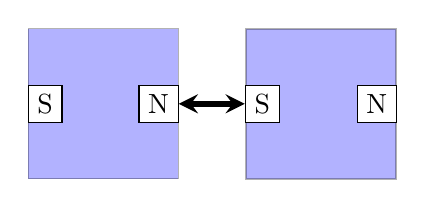
\begin{tikzpicture}

\node[fill=blue,opacity=.3,draw=black,minimum width= 0.75 in , minimum height= 0.75 in] (leftmag) at (0,0) {};
\node[anchor=center] (a) at (leftmag.east) {};
\node[anchor=center] (b) at ($(leftmag.east)+(0.33 in,0in)$) {};
\draw[stealth-stealth,line width=.07 cm] (a.center) -- (b.center); 
\node[anchor=west,opacity=.3,draw=black,fill=blue,minimum width= 0.75 in , minimum height= 0.75 in,draw=black,thick] (rightmag) at (b.center) {};

% \node[anchor=south] at ($(a)!0.5!(b)$ ) {x};

% label north and south
\node[anchor=east,fill=white,draw=black] at (leftmag.east) {N};
\node[anchor=west,fill=white,draw=black] at (leftmag.west) {S};
% label north and south
\node[anchor=east,fill=white,draw=black] at (rightmag.east) {N};
\node[anchor=west,fill=white,draw=black] at (rightmag.west) {S};



\end{tikzpicture}

\end{document}